\chapter{Methods to include environmental impacts in Australian health technology assessment}
\label{ch-9}

\begin{refsection}[refs/ch-9.bib]

The aim of this chapter was to outline the current Australian policy context for including environmental impacts in health technology assessment, evaluate potential methods to include environmental impacts in HTA for public reimbursement, and detail a method for use in the cost-minimisation pathway. This chapter contains the same text as a manuscript being prepared for submission. It summarises previous chapers for a policy audience and is partially based on concepts developed for an Issues Brief published by the Deeble Institute for Health Policy Research, which is provided in Appendix \ref{ap-i}.

\paragraph*{Publication details}
Manuscript authored by Jake T W Williams, Katy J L Bell, Scott McAlister, Madeleine Skellern, Rebecca Haddock, and Rachael L Morton. It is being prepared for submission.

\clearpage

\section{Introduction}
Health technology assessment (HTA) is a multidisciplinary process used in health systems to evaluate new health technologies including pharmaceuticals, tests, devices, vaccines, procedures, programs, or systems. The objective of HTA is to ensure new technologies provide health (or other) benefits at a cost acceptable to society.\cite{orourke_new_2020} In Australia, HTA is used to inform decisions about whether a new technology should receive publicly funded reimbursement, and environmental impacts are not currently considered during this process. However, there is interest in understanding if this should be done and how it could be implemented. The aim of this article is to: (1) outline the current Australian policy context relevant for including environmental impacts in HTA; (2) evaluate potential methods to include environmental impacts in Australian HTA for public reimbursement; and (3) detail one potential method for the Australian cost-minimisation pathway. 

\section{Australian Health Technology Assessment}
HTAs conducted globally usually include assessments of the technology’s safety, efficacy, clinical effectiveness, cost-effectiveness, and affordability; and may include other factors such as patient, caregiver, and clinician acceptability , health equity, ethical issues, and feasibility of implementation.\cite{world_health_organization_2015_2015} They do not currently consider environmental impacts. 

In Australia, most funding for healthcare comes from government sources, and two thirds of this comes from the Commonwealth Government.\cite{australian_institute_of_health_and_welfare_health_2024} While healthcare is also funded at other levels of government (e.g., by states and territories) and by individuals and households (e.g., for private services that do not receive reimbursement), HTA is used most prominently by the Commonwealth Government to inform decisions about which technologies are subsidised through one of Australia’s universal access schemes, such as the Pharmaceutical Benefits Scheme (PBS) or Medicare Benefits Schedule (MBS), as well as the level of the reimbursement provided. HTAs for this purpose are notably evaluated by the Pharmaceutical Benefits Advisory Committee (PBAC) and Medical Services Advisory Committee (MSAC). Guidelines for HTA submitted by applicants to MSAC for evaluation explicitly permit environmental impacts to be considered (Box 1),\cite{australian_government_department_of_health_disability_and_ageing_guidelines_2021} but this is not a requirement and it is unknown how often this information is submitted as part of an application. HTA submitted by applicants to the PBAC do not explicitly permit environmental impacts to be considered.\cite{australian_government_department_of_health_disability_and_ageing_guidelines_2016}

The Commonwealth Government is considering reforms to Australia’s HTA processes in response to the Health Technology Assessment Policy and Methods Review (henceforth HTA Review), published in 2024.\cite{australian_government_department_of_health_and_aged_care_health_2024} The HTA Review’s final report included a recommendation (Recommendation 43) to investigate options to include environmental impacts in HTA processes. This recommendation built on a related commitment in the 2023 National Health and Climate Strategy (Box 1).\cite{australian_government_department_of_health_and_aged_care_national_2023} The broader HTA policy context therefore presents a timely opportunity for Australia to progress this work. There is also international interest in this topic, with HTA bodies in the United Kingdom and Canada exploring ways to include environmental impacts in HTAs conducted in their health systems (Box 2). Despite this recent work, no jurisdiction routinely considers environmental impacts during HTA. 

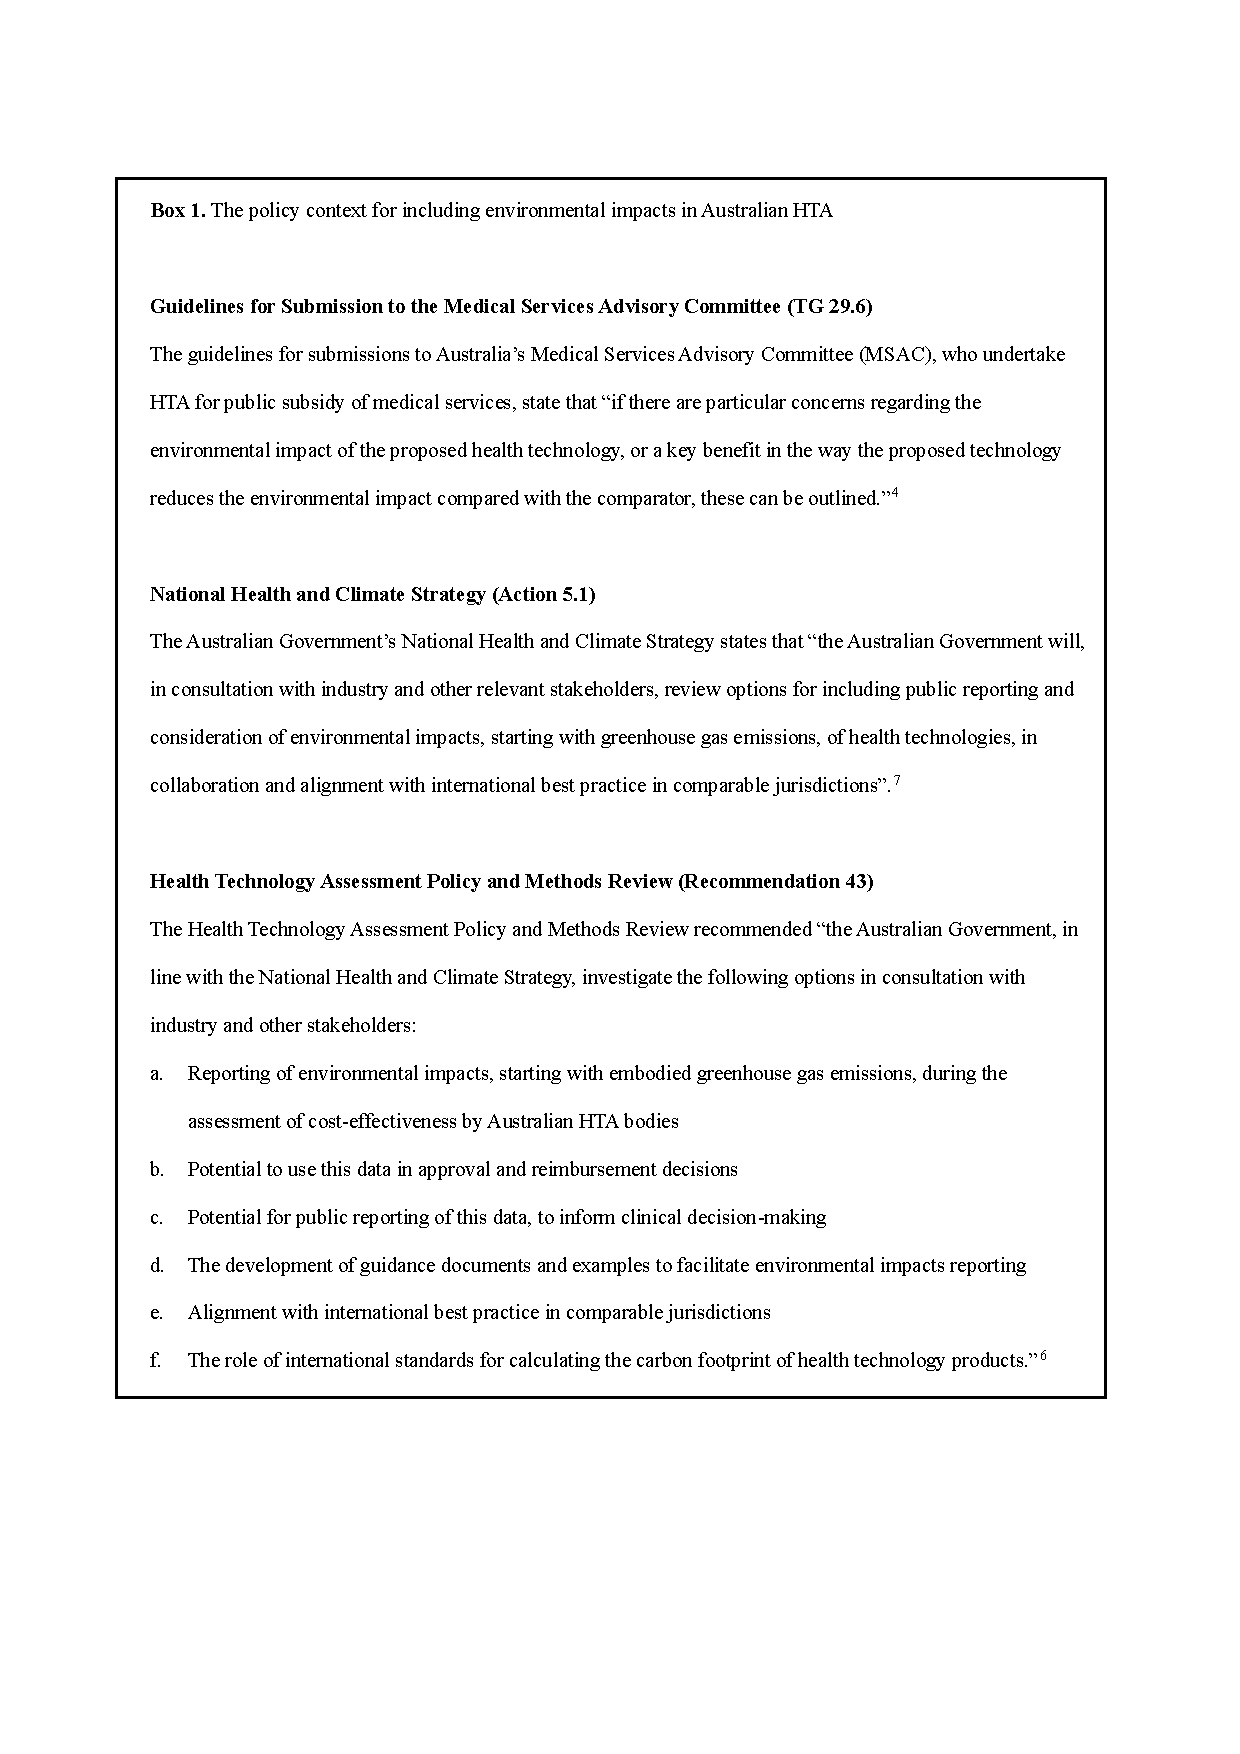
\includepdf[pages=-]{core-chapters/ch-9-box.pdf}

\section{Methods to include environmental impacts in HTA}
There is a growing literature dedicated to identifying, describing, and evaluating methods to include environmental impacts in HTA.\cite{guirado-fuentes_main_2023, toolan_environmental_2023, marsh_expanding_2016, desterbecq_inclusion_2023, mcalister_incorporating_2022, pinho-gomes_incorporating_2022, williams_methods_2024, ardito_which_2025} In this section we outline four broad methods and evaluate their potential use in Australia: (1) information conduit, (2) integrated evaluation, (3) parallel evaluation, or (4) environment-focused evaluation.\cite{toolan_environmental_2023}

\subsection{Information conduit}
An information conduit approach proposes the collection and publication of environmental impact data, but without using these data in the approval and reimbursement decision-making process. The applicant would submit environmental impact data for the proposed technology and the comparator, and the HTA body would make these data publicly available but would not use them to inform its recommendations. In Australia, this could be implemented by MSAC or PBAC as part of applications for reimbursement and submission of these data could be made either voluntary or compulsory. The information could be shared in the public summary document alongside the HTA outcome, or in another purpose-built repository or document for environmental impact information. This is different to the approach currently taken by MSAC, where environmental impacts can (hypothetically) be used to inform decisions, and where these data are not made publicly available.

The main advantage of this approach is that it could make substantial amounts of environmental impact data public, especially if providing the data were compulsory. These data could then be used by clinicians, patients, and researchers to inform individual clinical decisions. This information may be useful for clinical research and could be used to inform efforts to improve health outcomes while reducing environmental impacts. Compared with approaches that make use of environmental impact data in societal decision-making (which are described in the following sections), the information conduit approach may be an inefficient way to address the environmental impacts of new technologies if the goal of doing so is to minimise the use of products with high environmental impacts. 

\subsection{Integrated evaluation}
An integrated evaluation approach involves fully integrating environmental impacts into the HTA by identifying or creating new summary measures that allow clinical, financial, and environmental information to be synthesised into a single quantitative analysis.\cite{toolan_environmental_2023} In standard economic evaluations of health technologies costs and health benefits of alternative treatment options are quantified . In these evaluations environmental impacts can be integrated as either a cost or a benefit of the technology. For example, in relation to climate change impacts (one environmental impact of particular policy interest), greenhouse gas emission can be integrated into the measure of costs using a price or cost of a tonne of emissions, while it can be integrated into the measure of benefit using a value of health impact, such as quality adjusted life years,\cite{ducrot_integrating_2025} per tonne of emissions.

HTAs considered by MSAC and PBAC rely on information from cost-effectiveness (CEA) or cost-utility (CUA) analyses to inform their decisions.\cite{australian_government_department_of_health_disability_and_ageing_guidelines_2021, australian_government_department_of_health_disability_and_ageing_guidelines_2016} Cost-minimisation analyses (CMA) are accepted if the proposed technology has equivalent health impacts, and cost-benefit analyses (CBA) are not accepted.\cite{australian_government_department_of_health_disability_and_ageing_guidelines_2021, australian_government_department_of_health_disability_and_ageing_guidelines_2016} Because only CEA, CUA, and CMA are accepted, including environmental impacts on the benefits side of the analysis is only currently possible if environmental impacts can be valued as health outcomes in health units. 

A method to integrate future health damages induced by greenhouse gas emissions into quality-adjusted life years (QALY) was recently proposed using a conversion factor of 1.18×10−5 QALYs per kilogram of carbon dioxide equivalent.\cite{ducrot_integrating_2025} This amount represent the QALYs lost from emissions today. It is integrated into the CEA by deducting it from the QALYs gained from the technology. A conversion factor from greenhouse gas emissions to disability-adjusted life years (DALY) has also been demonstrated but this is less useful in the Australian context.\cite{tang_development_2018}

However, it has been argued that environmental impacts are more appropriately integrated as a cost not a benefit.\cite{hensher_incorporating_2020} While there is no consensus about this fact, there are more examples in recent literature, including from Australia, that integrate carbon emissions as a cost than as a health outcome.\cite{de_preux_beyond_2018, dunbar_balancing_2025} This method requires that environmental impacts be converted into monetary units. 

Environmental impacts can be valued in monetary units in two ways: using either a ‘damage cost ’ or ‘target consistent’ approach.\cite{aldy_keep_2021, nsw_government_carbon_2024} The damage cost approach monetises the damage to society of additional carbon emissions. A commonly used example of this is the social cost of carbon (SCC), such as the one proposed by the Australian Capital Territory Government.\cite{australian_capital_territory_government_act_2019} The SCC is estimated by modelling future carbon emissions, their effects on the climate, the resulting societal impacts of those climatic changes, and the monetary value of damages from the climatic changes. SCCs have also been estimated by the World Bank, International Monetary Fund, and, until recently, the United States.\cite{hensher_incorporating_2020} 

The target consistent approach values emissions at the marginal abatement cost of achieving defined emissions reduction targets, and not total societal damages. This approach is used by the New South Wales (NSW) Government to estimate their carbon values for CBA.\cite{nsw_government_carbon_2024} The current NSW emissions reduction targets are 50\% by 2030, 70\% by 2035, and net-zero by 2050, compared to 2005 levels. The NSW Government has set carbon values of \$130 per tonne in 2025 and \$350 per tonne in 2050 (in 2024 Australian Dollars) based on modelling of the implicit carbon price required to achieve emissions reductions aligned with the agreed target. 

Integrated evaluations could be requested by MSAC and PBAC by asking applicants to integrate environmental impacts in the cost-effectiveness information provided in their submissions , and this could be compulsory or voluntary. If done, guidance would be needed about which emissions should be included, over what period, and using which discount rate, questions that have not been fully explored in the published literature.

An integrated approach would not require any major changes to the HTA agency’s evaluation of cost-effectiveness or the interpretation of the application, as the environmental information would be converted into either health benefits or costs and integrated into the economic information that is supplied to the agency, such as the ICER. The evaluation of that ICER would remain the same. Though it is an open question whether ICER approval thresholds should be altered if environmental impacts are incorporated into the analysis. This may be less of an issue in Australia, where approval thresholds are not made explicit, than in countries where the HTA agency announces an approval threshold or band. 

There are a number of limitations with integrated evaluations. First, research suggests monetary conversions often undervalue the damages to society caused by climate change.\cite{rennert_comprehensive_2022} Target consistent approaches, such as the NSW carbon value, are inherently political and are based on current emissions reductions targets. These targets may change, or be abolished altogether, with changes in government or political will. Conversions to health outcomes are similarly uncertain and are likely to result in large confidence intervals due difficulties predicting the long-term health impact of carbon emissions.\cite{ducrot_integrating_2025}

Second, the value of environmental impacts as a cost in an economic evaluation are often much lower than the value of other health system costs included in the evaluation. Several examples of this phenomenon exist in the literature, including from Australia, which suggest that when valued in monetary units, environmental impacts account for a very small proportion of the total cost (less than a few percentage points) and are unlikely to influence reimbursement recommendations.\cite{de_preux_beyond_2018, dunbar_balancing_2025, pugliesi_cost_2025, williams_healthcare_2025} The exception to this may be when one healthcare technology has a much higher environmental impact than the other, such as with metered dose inhalers compared with dry powder inhalers for asthma care.\cite{hensher_incorporating_2020}

Recent work to describe the mortality accounting social cost of carbon (mSCC) found much higher values of greenhouse gas emissions, magnitudes higher than other estimates of the social costs of carbon.\cite{ducrot_integrating_2025} The mSCC should be explored further for use in Australia and has the potential to address these two key limitations. 

\subsection{Parallel evaluation}
A parallel evaluation approach involves HTA bodies analysing and presenting environmental impacts separately to costs and health gains . This information would then be considered during the HTA alongside clinical, economic, and other factors.\cite{toolan_environmental_2023} This approach does not attempt to synthesise environmental, cost, and health outcomes into a single metric, as with the integrated approach. Here, environmental impacts would be considered in parallel to other factors during the HTA. 

In its simplest form, a parallel evaluation involves considering environmental impacts during HTA agency deliberations. This method appears to be favoured by Canada’s Drug Agency,\cite{greenwood_dufour_how_2022} and this style of deliberative decision making is already used in Australia by MSAC and PBAC and their relevant sub-committees when considering clinical and economic factors. Given MSAC currently allows environmental impacts to be considered during their assessments (Box 1), it is assumed that this is how such considerations could currently be undertaken. Environmental impacts of a technology could either be considered by existing committees, or by new sub-committees dedicated to environmental considerations.

A limitation of this approach is that it places the onus of understanding and interpreting environmental outcomes on the members of the HTA committee, who do not usually have experience interpreting this type of data. This could be addressed by expanding the committees to include environmental scientists and by providing training to other members. However, a more important limitation of this approach is in how it deals with the weight of environmental factors relative to other factors and whether this weight reflects society’s preferences. Multi-criteria decision analysis (MCDA) is a method that makes the weight of the different factors involved in a decision explicit, reflecting the relative preferences of stakeholders. While MCDA has been used internationally in various healthcare contexts,\cite{thokala_multiple_2016, marsh_multiple_2016} and has been piloted for HTA in Queensland,\cite{howard_multicriteria_2018} it is not currently used in Australia for market authorisation or public subsidy. A recent study demonstrated methods to include carbon emissions in a MCDA.\cite{kingma_exploring_2025}

A final method that has been proposed as a parallel approach is to explicitly state the relationship between environmental impacts and health outcomes or costs.\cite{kindred_exploratory_2024} Kindred at al. have proposed two summary measures to achieve this: the incremental carbon footprint cost ratio (ICFCR) and the incremental carbon footprint effectiveness ratio (ICFER), which describe these relationships and are designed to be reported and interpreted parallel to the incremental cost-effectiveness ratio.\cite{kindred_exploratory_2024} The usefulness of these ratios is limited without additional work to understand preferences for the use. Additionally, the interpretability of these measures when reported alongside the conventional incremental cost-effectiveness ratio has not been investigated. Finally, operationalisation of Kindred et al.’s new summary measures would require consideration of uncertainty in the incremental carbon footprint, how this is correlated with the confidence intervals around incremental health gains and incremental costs, and how this affects the confidence intervals around the summary measures – a potentially methodologically involved topic. 

\subsection{Environment focused evaluation}
An environment-focused evaluation approach would require bodies conducting HTA to assess the value of technologies that are not expected to have any health benefits or cost savings. In these instances, the evaluation could focus on environmental impacts only.\cite{toolan_environmental_2023} This approach arguably has some precedent in Australia, where MSAC and PBAC can rely on cost information only (in the form of a cost-minimisation analysis) if there is evidence of no expected differences in health outcomes between the proposed technology and its comparator. This approach could theoretically be extended to allow bodies to only consider environmental impacts if there is evidence of no expected difference in health outcomes or expected differences in costs between the proposed technology and its comparator. This would be separate to the current cost-minimisation pathway. Requiring HTA bodies to evaluate technologies with no health or cost benefits would represent a major shift in the type of technologies assessed during Australian HTA.

\section{A decision matrix for Australian cost-minimisation analysis }
Two methods are likely to be immediately useful in the Australian context. The first is to integrate environmental impacts in a cost-effectiveness or cost-utility analysis. This method does not require major changes to the HTA deliberative process and may be the method implied by the HTA Review, which recommends the consideration of environmental impacts during the assessment of cost-effectiveness. Decision maker preferences for this method in Australia have not been explored, but there is an increasing number of examples in the literature that report its application. The second is to assess environmental impacts parallel to other relevant factors during the deliberative HTA process. This method does not require changes to established economic evaluation methods, may already permitted for MSAC HTA, and may be consistent with international approaches. This parallel approach might be conveniently introduced in Australia in the context of cost-minimisation analyses, where health outcomes are assumed to be equivalent. 

Focusing on the CMA pathway is beneficial because it avoids potentially unacceptable trade-offs between health and the environment. These trade-offs may be introduced when a technology has potential health benefits that are being considered alongside environmental impacts. Preliminary work from the UK suggests a degree of public support for HTA recommendations that approve technologies with lower environmental impacts but higher costs – but preferences for technologies with lower environmental impacts but lower health gains have not directly been tested, and are less likely to be acceptable.\cite{nice_nice_2023}

The nine possible scenarios when incremental health gains are zero are outlined in the decision matrix presented in Figure \ref{fig:ch-9-fig-1}. The most certain scenarios arise where both costs and environmental impacts are lower (Scenario A – a “win-win”) or higher (Scenario I – “lose-lose” technologies). Certain decisions can also be made in scenarios where environmental impacts are equivalent and costs are lower (Scenario D) or higher (Scenario F). In these four scenarios, environmental impacts are used to reinforce the decision that would have been made based on the interpretation of cost information alone.

\begin{figure}
    \centering
    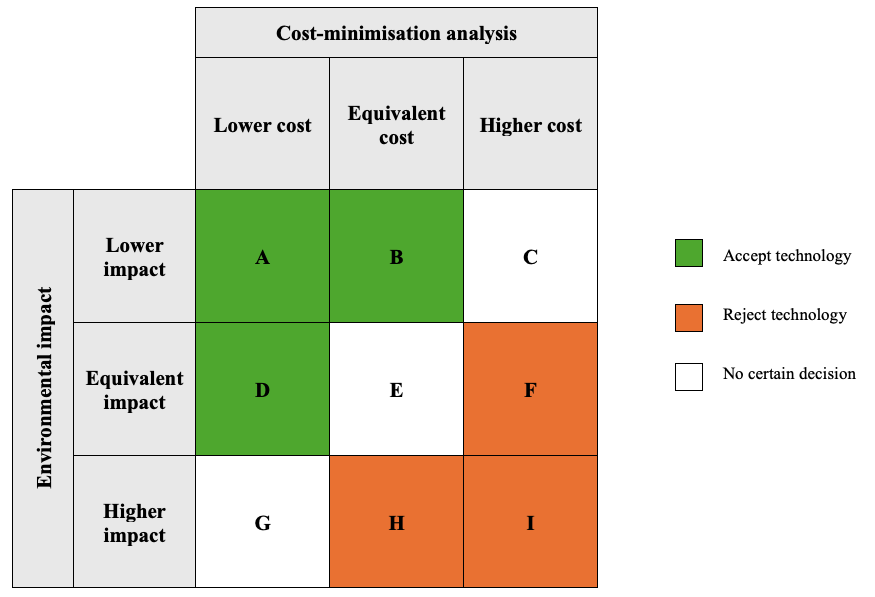
\includegraphics[width=1\linewidth]{core-chapters/figs/ch-9-fig-1.png}
    \caption{Decision making matrix for cost-minimisation analysis and environmental impacts, assuming acceptability of trade-offs between costs and carbon emissions.}
    \label{fig:ch-9-fig-1}
\end{figure}

Decisions might also be made when the proposed technology has equivalent costs and lower or higher environmental impacts. In these scenarios, environmental outcomes can be used as a decision modifier to either accept (Scenario B) or reject (Scenario H) the technology. These two decisions are environment-focused in their approach as they deal with technologies that are not expected to have health or cost benefits. 

The socially optimal decision is less certain in the remaining three scenarios. Two of these occur when the proposed technology has lower environmental impacts but higher costs (Scenario C), or higher environmental impacts but lower costs (Scenario G). There has been very little research undertaken to understand public perspectives about these types of trade-offs, and no work has been undertaken in the Australian context. The final scenario is when both the cost and environmental outcomes – as well as the health gains – are neutral (Scenario E). In this case, the HTA agency would need to look at other factors to make a recommendation. 

The benefit of the decision matrix in Figure 1 is that it makes explicit how and when environmental impacts might be considered by an HTA agency – something that is not generally clear in the parallel evaluation approach. It also does not rely on MCDA or the identification of explicit weighting of criteria and may therefore be acceptable and easier to implement in Australian where there is no precedent for using MCDA in HTA.

\section{Future research and conclusions }
If environmental impacts are to be considered routinely in Australian HTA, several outstanding challenges that need to be addressed. These include methodological issues related to integrated evaluations, such as discount rates, willingness-to-pay thresholds, and whether impacts should be considered a cost or benefit. Methods are also limited by a lack of knowledge about societal preferences concerning the trade-off between health outcomes, costs, and environmental impacts.

One potential limitation of considering the environmental impacts of health technologies through formal HTA pathways is that HTA is only undertaken for new technologies. Any move to consider environmental impacts in HTA should therefore ideally be accompanied by measures over time to also consider the environmental impact of already approved health technologies, which constitute a high proportion of spending. While HTA bodies do not currently review already approved technologies, the HTA Review recommends the Australian Government update post-review frameworks for evaluation (Recommendation 18), opening an opportunity to also consider environmental impacts in this process. 

In this article we have outlined the current Australian policy context, evaluated potential methods in the Australian context, and proposed a simple decision matrix to guide the parallel interpretation of environmental impacts alongside cost-minimisation analysis. We do not propose this method as a complete solution to the challenges of including environmental impacts in HTA. Instead, we propose it as a relatively simple and effective starting point for developing a more comprehensive methodological approach to considering environmental impacts in Australian HTAs. \textcolor{white}{\cite{national_institute_for_health_and_care_excellence_hta_nodate} \cite{noauthor_health_2025} \cite{canadian_agency_for_drugs_and_technologies_in_health_health_2015} \cite{benard_environmental_2025} \cite{canadas_drug_agency_ahead_2022}}

\printbibliography[heading=subbibliography]
\end{refsection}